\documentclass[sigplan,nonacm,anonymous,review]{acmart}

\usepackage{authorcomments}
\usepackage{listings}
\usepackage{algorithm}
\usepackage{algpseudocode}
\usepackage{xspace}
\usepackage{paralist}


\lstset{language=R}
\definecolor{LightGray}{rgb}{.92,.92,.92}
\definecolor{Gray}{rgb}{.3,.3,.3}
\definecolor{DarkGray}{rgb}{.5,.5,.5}
\lstset{ %
  columns=flexible,
  captionpos=b,
  frame=single,
  framerule=0pt,
  tabsize=2,
  belowskip=0.5em,
  backgroundcolor=\color{LightGray},
  basicstyle=\small\ttfamily,
  emphstyle=,
  keywordstyle=,
  commentstyle=\color{Gray}\em,
  stringstyle=\color{Gray},
  numbers=left,
  showstringspaces=false
}
\lstdefinestyle{R}{ %
  language=R,
  morekeywords={assign, delayedAssign},
  deletekeywords={env, equal, c, runif, trace, args, exp, t, all},
  breaklines=true
}
\lstdefinestyle{Rin}{ %
  style=R,
  breaklines=false
}


\newcommand{\tool}{\texttt{signatr}\xspace}
\newcommand{\numFnsCaseStudy}{20\xspace}
\newcommand{\numPkgsScaleStudy}{20\xspace}
\newcommand{\code}[1]{{\lstinline[style=Rin]!#1!}\xspace}

% For algorithmcx
\algnewcommand{\LineComment}[1]{\State \(\triangleright\) #1}
\newcommand{\DBFileSize}{287.17 GB\xspace}
\newcommand{\DBValuesRnd}{39.4M\xspace}
\newcommand{\DBValues}{39,425,582\xspace}
\newcommand{\DBNumPackagesRnd}{652\xspace}
\newcommand{\DBNumPackages}{652\xspace}
\newcommand{\DBNumFunctionsRnd}{38.1K\xspace}
\newcommand{\DBNumFunctions}{38,109\xspace}
\newcommand{\DBNumSourceFilesRnd}{17.5K\xspace}
\newcommand{\DBNumSourceFiles}{17,463\xspace}
\newcommand{\DBSourceLinesOfCodeRnd}{389.7K\xspace}
\newcommand{\DBSourceLinesOfCode}{389,740\xspace}

\newcommand{\UFTracingBudgetRnd}{5K\xspace}
\newcommand{\UFTracingBudget}{5,000\xspace}
\newcommand{\UFNumTracesRnd}{12.1M\xspace}
\newcommand{\UFNumTraces}{12,115,000\xspace}
\newcommand{\UFNumSuccessTracesRnd}{2.1M\xspace}
\newcommand{\UFNumSuccessTraces}{2,062,046\xspace}
\newcommand{\UFRatioSuccessTraces}{17\%\xspace}
\newcommand{\UFNumPackagesRnd}{78\xspace}
\newcommand{\UFNumPackages}{78\xspace}
\newcommand{\UFNumFunctionsRnd}{2.4K\xspace}
\newcommand{\UFNumFunctions}{2,423\xspace}
\newcommand{\UFNumOfCrashedRSessionsRnd}{201\xspace}
\newcommand{\UFNumOfCrashedRSessions}{201\xspace}
\newcommand{\UFNumSuccessPackagesRnd}{69\xspace}
\newcommand{\UFNumSuccessPackages}{69\xspace}
\newcommand{\UFNumSuccessFunctionsRnd}{1.2K\xspace}
\newcommand{\UFNumSuccessFunctions}{1,228\xspace}
\newcommand{\UFNumFunctionSignatrSignatureRnd}{1.1K\xspace}
\newcommand{\UFNumFunctionSignatrSignature}{1,113\xspace}
\newcommand{\UFAvgNewSignatrSignatureRnd}{707.7\xspace}
\newcommand{\UFAvgNewSignatrSignature}{707.7\xspace}
\newcommand{\UFAvgNewSignatrSignatureRatioRnd}{213\xspace}
\newcommand{\UFAvgNewSignatrSignatureRatio}{213\xspace}
\newcommand{\UFBaselineSignaturesRnd}{8.3K\xspace}
\newcommand{\UFBaselineSignatures}{8,272\xspace}
\newcommand{\UFSignatrSignaturesRnd}{787.7K\xspace}
\newcommand{\UFSignatrSignatures}{787,696\xspace}
\newcommand{\UFSharedSignatureRnd}{834\xspace}
\newcommand{\UFSharedSignature}{834\xspace}
\newcommand{\UFSharedSignatureFunctionRnd}{432\xspace}
\newcommand{\UFSharedSignatureFunction}{432\xspace}
\newcommand{\UFSignatrBaselineSignaturesRatioRnd}{95.2\xspace}
\newcommand{\UFSignatrBaselineSignaturesRatio}{95.2\xspace}
\newcommand{\UFNumMissingFunctionSignatrRnd}{1.3K\xspace}
\newcommand{\UFNumMissingFunctionSignatr}{1,310\xspace}
\newcommand{\UFNumMissingFunctionSignatrRatio}{54.1\%\xspace}
\newcommand{\UFNumFunctionSignatrSignatureRatio}{45.9\%\xspace}
\newcommand{\UFNumFunctionBaselineSignatureRnd}{2K\xspace}
\newcommand{\UFNumFunctionBaselineSignature}{2,038\xspace}
\newcommand{\UFNumFunctionBaselineSignatureRatio}{84.1\%\xspace}
\newcommand{\UFNumErrorMessagesRnd}{789.9K\xspace}
\newcommand{\UFNumErrorMessages}{789,896\xspace}

\newcommand{\TRTracingOverhead}{7.8\xspace}
\newcommand{\TRTracingFilesRnd}{3.2K\xspace}
\newcommand{\TRTracingFiles}{3,236\xspace}
\newcommand{\TRAvgTracingOverhead}{3.3\xspace}
\newcommand{\TRMaxTracingOverhead}{7.8\xspace}
\newcommand{\TRMinTracingOverhead}{1.2\xspace}
\newcommand{\TRTracingBudgetRnd}{5K\xspace}
\newcommand{\TRTracingBudget}{5,000\xspace}
\newcommand{\TRTracesSize}{353.55 MB\xspace}
\newcommand{\TRTracesReturnDbsSize}{58.39 GB\xspace}
\newcommand{\TRNumTracesRnd}{12.1M\xspace}
\newcommand{\TRNumTraces}{12,115,000\xspace}
\newcommand{\TRNumSuccessTracesRnd}{2.1M\xspace}
\newcommand{\TRNumSuccessTraces}{2,062,046\xspace}
\newcommand{\TRRatioSuccessTraces}{17\%\xspace}
\newcommand{\TRNumPackagesRnd}{78\xspace}
\newcommand{\TRNumPackages}{78\xspace}
\newcommand{\TRNumFunctionsRnd}{2.4K\xspace}
\newcommand{\TRNumFunctions}{2,423\xspace}
\newcommand{\TRNumOfCrashedRSessionsRnd}{201\xspace}
\newcommand{\TRNumOfCrashedRSessions}{201\xspace}
\newcommand{\TRNumSuccessPackagesRnd}{69\xspace}
\newcommand{\TRNumSuccessPackages}{69\xspace}
\newcommand{\TRNumSuccessFunctionsRnd}{1.2K\xspace}
\newcommand{\TRNumSuccessFunctions}{1,228\xspace}



\begin{document}

\title{\tool: A Data-Driven Fuzzing Tool for R}

\begin{abstract}
The fast-and-loose, permissive semantics of dynamic programming
languages limit the power of static analyses. For that reason, soundness is often
traded for precision through dynamic program analysis.  Dynamic
analysis is only as good as the available runnable code, and relying
solely on test suites is fraught as they do not cover the full gamut of
possible behaviors. Fuzzing is an approach for automatically
exercising code, and could be used to obtain more runnable code.
However, the shape of user-defined data in dynamic languages is
difficult to intuit, limiting a fuzzer's reach.  

We propose a feedback-driven blackbox fuzzing approach which draws inputs from a
database of values recorded from existing code.  We implement this
approach in a tool called \tool for the R programming language.  We
present the insights of its design and implementation, and assess
\tool's ability to uncover new behaviors by fuzzing \UFNumFunctions R
functions from \UFNumPackages R packages, revealing
\UFSignatrSignatures new signatures.
\end{abstract}

\maketitle

\section{Introduction}\label{sec:introduction}

Dynamic analysis is often the only practical way to analyse code
written in dynamic languages as the semantics of these languages
renders static analyses useless.  Dynamic analysis, however, requires
both code to run and valid inputs for said code. To draw conclusions
about a code base, one could run the existing, runnable code, \Eg,
tests, but such code paints an incomplete picture as it is challenging
to fully cover the range of behaviors allowed by the permissive
semantics of dynamic languages.

To increase coverage, one could make use of a \textit{fuzzer}, a tool
that exercises code by generating random inputs.  Fuzz testing is
popular and has seen widespread adoption, primarily to find bugs,
performance pathologies, and security vulnerabilities.  However,
dynamically languages such as Python, JavaScript, and R pose unique
challenges that revolve around the idea that \textit{dynamic code
  tends hide runtime errors}.  For instance, accessing a non-existent
field of an object in JavaScript yields the value {\tt undefined}
instead of crashing, and basic functions in R will readily coerce
values whose types do not match.  A tool that tries to run code
automatically will thus have very little to go on vis-\`a-vis the
correctness of the code being generated as there is no clear
observable witness of an error. On top of this, the lack of static
types leaves fuzzers with very little information about what values
are expected to begin with. Finally, it is difficult to generate complex
values automatically in dynamically typed languages; in a statically typed language like Java, the
shapes of user-defined objects can be inferred from a static class
definition. In contract, there is no such guide in dynamic languages, limiting
a fuzzer's ability to generate realistic inputs.

To get around this, we propose an approach to fuzzing that relies on
an extensive database of observed values.  We develop a tracer that
collects information about function calls and values created during
code execution, and store this information in a database with an
expressive query API. Then, we leverage this database to generate
new function calls using the recorded values.  This approach is
implemented in a tool called \tool for the R programming language.

To validate our tool, we revisit an application of dynamic analysis,
namely trace typing~\cite{andreasen2016trace} where the goal is to guess
the signatures of library functions by observing the values that they
accept and return. We perfom that experiment on R libraries and use
the {\tt contractr} type inference tool~\cite{turcotte2020designing},
wherein function types were inferred from recorded calls in R package
test, example, and vignette code.  Fuzzing \UFNumFunctions of those R
functions with our tool generated \UFSignatrSignaturesRnd new unique
signatures compared to the original study.

In summary, our contributions are:
\begin{inparaenum}[(1)]
\item a fuzzing technique relying on a database of observed values;
\item an implementation of this approach in a tool for R; and
\item a use case where we generate yet unseen signatures.
\end{inparaenum} 
Our tool is open source and is available online alongside the data set
used here.

\section{Background and Related Work}
\label{sec:background}

\paragraph{Related Work}
We explore an approach to fuzzing where no input is required from the
programmer.  Out of the many fuzzers, we have experience with Randoop,
a feedback-driven random test generation tool for
Java~\cite{pacheco2007randoop}.  Essentially, sequences of method
calls are generated to test classes, and arguments are randomly
generated for these calls. For primitive values, a random value is
selected from a predefined, but user-extensible list; for reference
types a value is selected at random from those which have been seen,
and if none are available then {\tt null} is selected.  While this
technique is effective at generating tests involving non-trivial
objects that are built up from a number of method calls, data science
languages like R oftern require generating realistic data.  QuickCheck
is another interesting tool in this space~\cite{quickcheck}.  While it
can generate random inputs, the strategy for constructing inputs needs
to be specified.  The lack of type information in R limits the
usefulness of such approaches. American Fuzzy Lop (AFL) is a
state-of-the-art industrial fuzzer~\cite{afl}. AFL takes a program and
one example file as input, calls the program with the input, and then
uses a variety of heuristics to transform the input and fuzz the
program.  AFL aims to find defects, looking for edge cases.  Our
approach on the other hand looks for calls that do not crash, and
discovers new acceptable inputs.

\paragraph{The R Programming Language}

We present a fuzzing tool called \tool for R, a language which sports an unusual mix of
language features making it a challenging target for
tooling~\cite{morandat2012evaluating}.  Challenges include:

\begin{compactitem}[$-$]
\item The lack of type annotations or static type system; so there is
  little to suggest what are expected arguments or return values.
\item Primitive values (booleans, integers, ...)  have a separate
  ``NA'' value indicating that data is ``not available''.
\item Values are automatically and silently coerced across types.
  Each function may coerce parameters as it sees fit.
\item Most values are vectors and can be annotated by key-value pairs
  called \textit{attributes} (\Eg the \code{dim} attribute turns a vector into a matrix).
  Attributes coupled with reflection are
  the building blocks for advanced features such as
  object-orientation.  In R, there is no description of a shape of an
  object, it is simply a value with the \code{class} attribute.
\item Function arguments are evaluated lazily resulting in unpredictable
  ordering of side-effects.
\item Shared values are copied on write. A value is shared if it is
  accessible from multiple variables. Thus visible side effects are less
  frequent than in traditional imperative languages.
\end{compactitem}

\bigskip
There has been work on a static type system for
R~\cite{turcotte2020designing}.  A simple type annotation language has
been evaluated on a corpus of 400 R packages.  As part of our
assessment of \tool, we will revisit that work and demonstrate improvements
by discovering new signatures for the previously studied functions.

\section{Approach}

There are two main phases to our approach:
%
\begin{inparaenum}[(1)]
\item \emph{recording} R code as it runs; this involves capturing
  function arguments and return values in our value database, and
\item \emph{fuzzing} by drawing inputs to functions from the database.
\end{inparaenum}
This is pictured in Figures~\ref{fig:sxpdb-pipeline} and
\ref{fig:fuzz-pipeline} for the recording and fuzzing phases
respectively.

For the recording phase, runnable code is extracted from examples and
tests in packages.  This runnable code consists of a set of scripts
that can be run independently. Next, the scripts are
executed in parallel, and all arguments are recorded into separate instances of
our database, called the \sxpdb.  Finally, all the database instances
are merged into one, in the process duplicate values are discarded. GNU parallel is used for orchestration~\cite{tange2011_parallel}.

As for the fuzzing phase, a list of functions to fuzz as well as a
\sxpdb are taken as input. The functions are fuzzed in parallel.  The
output of the fuzzer is a list of successful function calls, where a
successful call is defined as one that generated no warnings, errors,
and did not cause R to crash.  The fuzzer relies on hooks before and
after function execution: the hook before invocation allows the fuzzer
to process inputs, and the hook after allows errors to be signalled
and handled and the return value to be processed.  The
after-invocation hook can also be used to expand the feedback given to
the fuzzer.  Concretely, the fuzzer runs the functions using an
extended R virtual machine that supports attaching callbacks to
various runtime events~\cite{goel2019}.  Users can also plug their own
dynamic analysis directly into the pipeline.

Since R can crash (and does), to avoid losing results each instance
of the fuzzer consists of two processes. A worker that fuzzes, and a
supervisor that can spawn workers if neeeded.  Furthermore, the fuzzer
runs isolated in a container as calling arbitrary code could have dire
consequences.

The tool iteself consists of three standalone components: \code{argtracer},
the tracer responsible for running code and recording function
invocation, \code{sxpdb}, the value database, and finally \code{generatr}, the
fuzzer responsible for generating inputs. They are R
packages written in combination of R and C++.

\begin{figure}
    \centering
    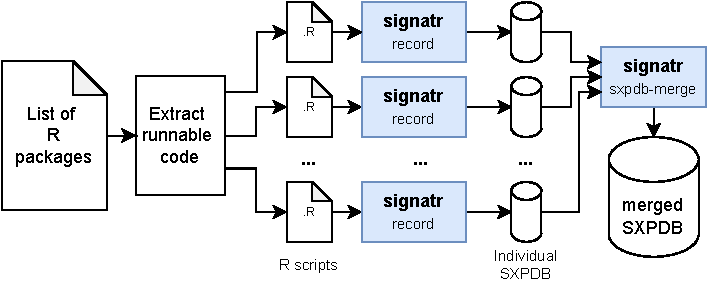
\includegraphics[width=\columnwidth]{code-and-figures/sxdb-pipeline.pdf}
    \caption{ Recording pipeline.  }\label{fig:sxpdb-pipeline}
\end{figure}

\begin{figure}
    \centering
    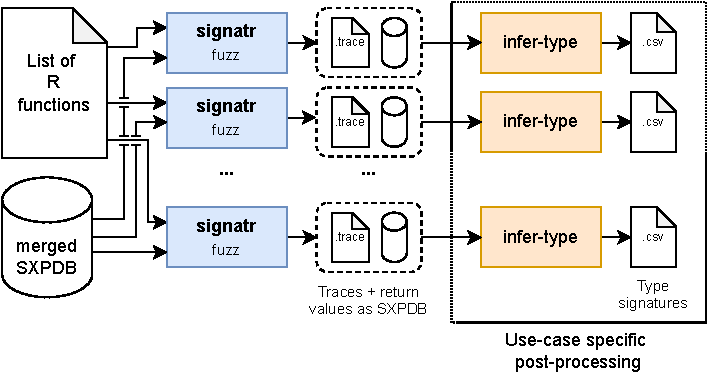
\includegraphics[width=\columnwidth]{code-and-figures/fuzz-pipeline.pdf}
    \caption{    Fuzzing pipeline.    }\label{fig:fuzz-pipeline}
\end{figure}

\subsection{Tracer}\label{sec:argtracer}

The tracer is built on top of aforementioned extended virtual machine.
The two runtime events we use are function exit, where all arguments are
captured and stored, and a context jump, which is necessary to keep
the call stack healthy as the interpreter uses long jumps for loop
control flow, return statements, and error handling.  (On a long jump,
the exit hook is ignored, so we maintain our own version of the call stack
to capture all function exits.)

When the tracer sees a call, it only sees a pointer to a closure, and the
function's name and its package can only be found by searching through
the loaded namespaces and the symbols they contain.  Because of this,
the tracer eagerly builds an index of package and function names when
namespace functions are loaded.

Regarding performance, there is \TRMinTracingOverhead ---
\TRMaxTracingOverhead (\TRAvgTracingOverhead on average) slowdown when
running with tracing enabled (based on the running / tracing
\TRTracingFiles R scripts recording 8M unique values of 3GB size).
This cost is mostly due to the value serialization.  The tracer is written in 600 lines of
C++ code.

\subsection{Database of Values}\label{sec:sxpdb}

The database is hand-written in order to leverage domain-knowledge of
R values, and optimize it for the queries supported by our API.  It is
implemented in 5K lines of C++ and 1.5K lines of R code.

\paragraph{Storage}


The database stores unique values.  We use XXH\-128 hashes for
uniqueness in combination with a hashtable based on RobinHood
hashing\footnote{\url{cyan4973.github.io/xxHash},
\url{github.com/martinus/robin-hood-hashing}}.  While the hashing is
fast, we need to lower R values into a binary format.  R provides a
binary serialization XDR, but it is
costly\footnote{\url{cran.r-project.org/doc/manuals/r-release/R-ints.html\#Serialization-Formats}}.
We also strip the serialization of sources of non-determinism related
to character encodings.  Since many values are pushed to the database
in an average recording session, we try to avoid serialization as much
as possible.  For this we use the \code{trace} bit that is part of
each value\footnote{A bit in the C struct that represents a value,
\url{cran.r-project.org/doc/manuals/r-release/R-ints.html\#Rest-of-header}.}.
If not set, the value is fresh and we serialize it, compute its hash,
store it. The trace bit is then set to avoid repeated serialization.
In spite of R's copy-on-write semantics, values can be modified in
place before being shared, and these values may be serialized repeatedly
to capture the updates performed by the program.

The database also store metadata about values and their origin.  We
also keep a unique id for each sequence of arguments coming from the
same call site. This allows us to replay the calls as they were
observed.

The database maintains tables for the hashes, runtime metadata (e.g.,
how often a value was seen), static metadata, origins, call ids, and
class names.  Variable length data, such as the serialized values, are
stored in a combination of 2 tables, one giving an offset into the
other table which holds the size of the value and the value itself.
Origin strings and class names are interned, i.e., each unique string
is stored separately, and referred to by pointer.  Search indices are
built using fast compressed bitsets~\cite{chambi2016better}.  The
database supports all values except external pointers (e.g. pointer to
C allocated data).  Environments and closures were not stored in the
database during our experiments since they dramatically increased
memory pressure.

Finally, opening the database in {read mode} only loads metadata.
Retrieving values from disk is done on demand, making it possible to
query larger-than-memory databases.

\paragraph{Queries}

Values can be queried based on their {\tt typeof}-type or class, on
the presence of NAs, number of attributes, and dimensions.  The database
can be queried for a random value with the desired metadata (e.g., query for a
vector of integers of length 10), or can be queried by providing an
existing value along with a list of search parameters to be relaxed
(e.g., query for a value similar to {\tt 42}, but relax
on the length).  A custom predicate can also be used to filter
returned values.

\subsection{Fuzzing}

The value database is at the core of our fuzzing approach, which is
similar in spirit to mutation-based fuzzing. Instead of mutating
arguments to previous calls, new argument values are selected based on
previous ones.

The fuzzer generates calls to a function and chooses arguments to these
calls as depicted in Algorithm~\ref{alg:arg-sel}.  In addition to the
target function and database, the algorithm considers how many query
parameters to relax on (\emph{numRelax}), as well as all of the
previously seen successful calls to the function (\emph{succs}).
For each parameter, the algorithm determines how to relax (this may
change from one iteration to the next), finds all values that
inhabited that parameter in successful calls, chooses one value, and
queries the database for a value similar to it save for the
relaxation.  If no successful calls to the function have been
observed, random values can be chosen.

The fuzzing approach itself is depicted in Algorithm~\ref{alg:fuzzer}.
First, the collection of already known calls to the function is obtained
from the database.  The main idea of the approach is to start by
selecting new arguments essentially at random by querying the database
and relaxing on many parameters, and gradually reduce the number of
parameters being relaxed as the fuzzer progresses.  Concretely, the
number of parameters being relaxed is reduced every \emph{tick},
which is determined by dividing the total fuzzing budget by the number
of parameters that can be relaxed (\emph{numRelaxParams}).  The
function will be fuzzed for as long as the budget allows, and
initially all database parameters will be relaxed.  Arguments for a
new call are generated through the approach depicted in
Algorithm~\ref{alg:arg-sel} (\emph{getArgs}), the call is performed,
and the results are saved in \emph{res}.  If there were no errors,
warnings, or crashes, then the successful call is added to the list of
successful calls \emph{succs} and iteration continues until the
budget is exhausted.

\begin{algorithm}
\caption{Selecting Arguments for New Call}\label{alg:arg-sel}
\begin{algorithmic}[1]
\Procedure{getNewArgs}{$f,numRelax,db,succs$}
\State{$params \gets getParameters(f)$}
\For{$p$ in $params$}
\LineComment{relax on $numRelax$ parameters}
\State{$relax \gets pickSome(relaxParameters, numRelax)$}
\LineComment{get all values that $p$ had in successful calls to $f$}
\State{$seed \gets getArgsFor(p, succs)$}
\LineComment{choose one at random}
\State{$v \gets pickOne(seed)$}
\LineComment{sample a similar value from the database}
\State{$args[p] \gets sampleSimilar(v, db, relax)$}
\EndFor
\State \textbf{return} $args$\Comment{the args for the new call}
\EndProcedure
\end{algorithmic}
\end{algorithm}

\begin{algorithm}
\caption{Fuzzing}\label{alg:fuzzer}
\begin{algorithmic}[1]
\Procedure{fuzzWithDB}{$f,db,budget$}
\State $succs \gets getSuccessfulCalls(f, db)$
\State $tick \gets budget / numRelaxParameters$
\State $relaxThisTime \gets numRelaxParameters$
\State $i\gets 1$
\While{$i\not=budget$}
\LineComment{gradually relax on fewer parameters}
\If{$i \bmod tick = 0$}
\State $relaxThisTime \gets relaxThisTime - 1$
\EndIf
\State{$args \gets getNewArgs(f,relaxThisTime, db, succs)$}
\State{$res \gets call(f, args)$}
\LineComment{add successful call to $succs$}
\If{no warnings, errors, crashes in $res$}
\State{$succs \gets succs + res$}
\EndIf
\State $i\gets i+1$
\EndWhile\label{endfuzzloop}
\State \textbf{return} $succs$\Comment{the successful calls to $f$}
\EndProcedure
\end{algorithmic}
\end{algorithm}

\section{Assessment}
\label{sec:assessment}


We used \tool to stress-test one of the proposed type system for
R~\cite{turcotte2020designing}.  The type system was designed
empirically, with the help of a dynamic analysis that inferred
function signatures from the types of values observed while running
extracted code from packages.  In a nutshell, a type was inferred from
each call to a function, and these types were unified into a single
function type, and the more unique successful calls there are, the
more precise the inferred signature---the types inferred from
successful calls are referred to as \textit{call signatures}.  It
would be therefore interesting to see \emph{how many additional
successful calls can \tool generate?}

We ran all of our experiments on two Ubuntu 18.04 servers, each with a
72 core Intel Xeon 6140 2.30GHz processor and 256GB of RAM.

\paragraph{Recording}

First, we created a \sxpdb for the fuzzer.
For this we used the extracted runnable code from the same corpus as the original study which consists of \DBNumSourceFiles R scripts containing \DBSourceLinesOfCodeRnd lines of code (excluding comments and new lines).
The database was generated in 16 hours and occupies \DBFileSize of disk space.
It contains \DBValuesRnd unique values recorded from \DBNumCallsRnd calls to \DBNumFunctionsRnd functions in \DBNumPackages packages.
Figure~\ref{fig:argsdb-value-distribution} shows the distribution of main value types.
The vast majority of values are vectors and matrices of real numbers which is unsurprising as R is mostly used for numerical computing.
That said, many of them (47.2\%) contain attributes which is what makes them interesting, as attributes add semantic meaning.
The next big group are lists, which can be divided into two groups, data frames (two dimensional, column-major structure representing observations) and records.


\begin{figure}
    \centering
    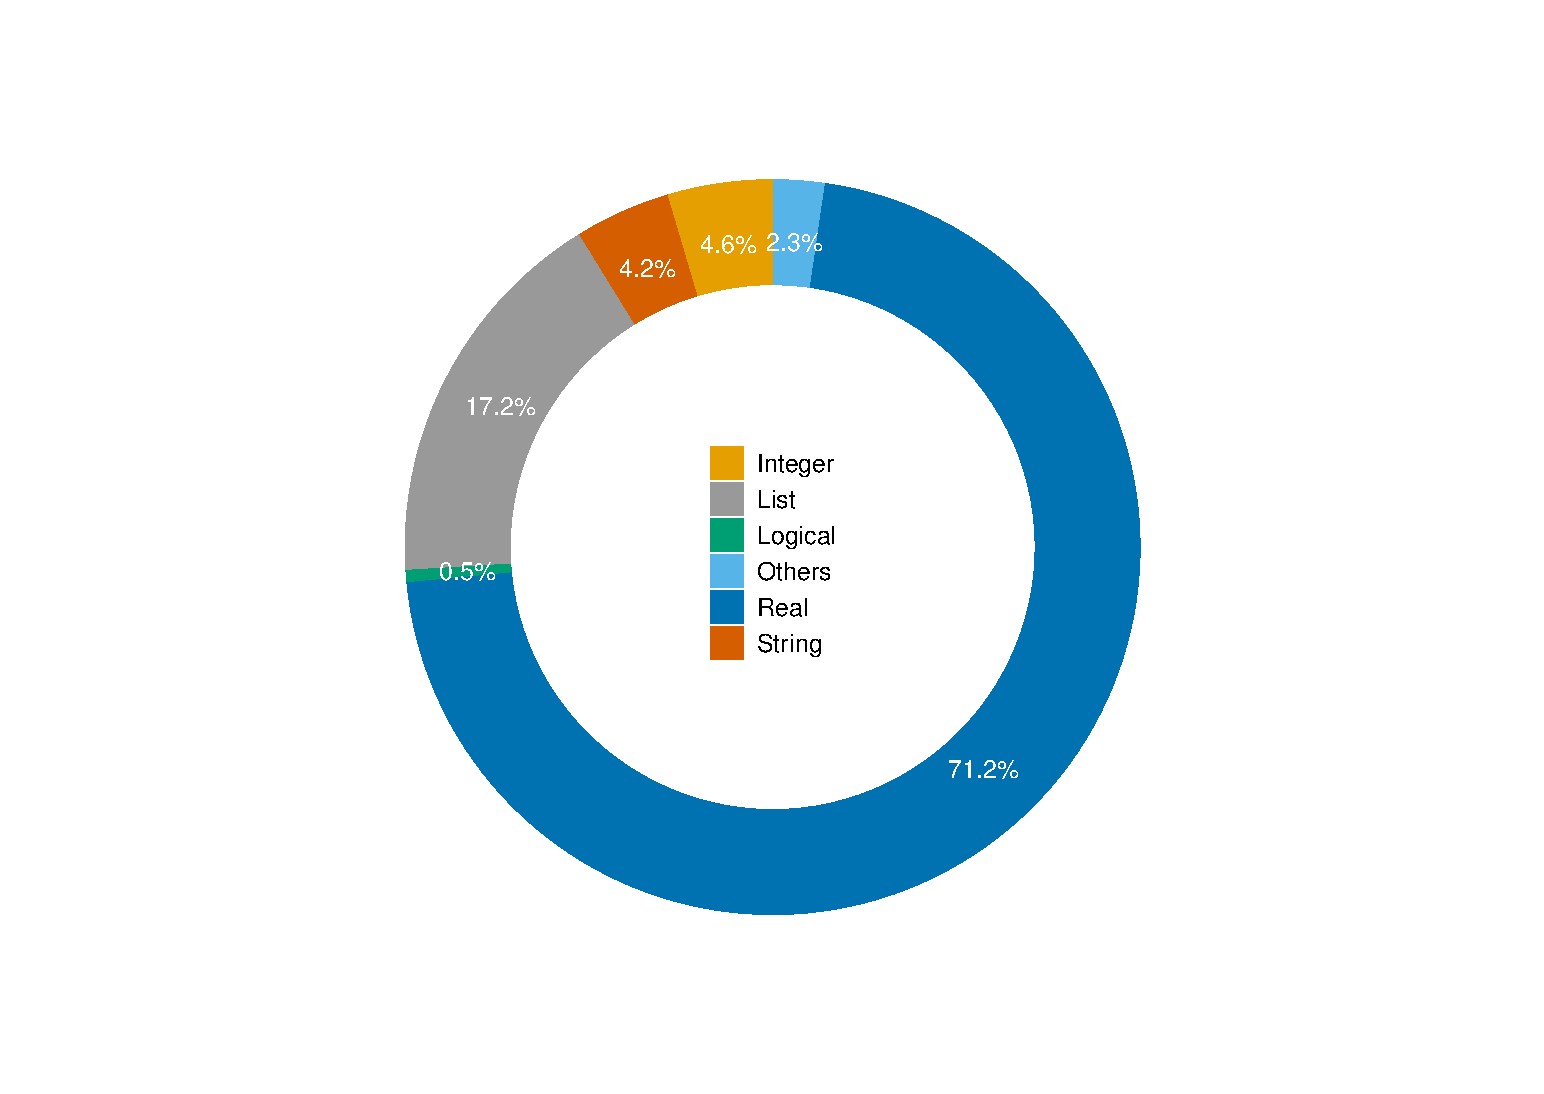
\includegraphics[width=.6\columnwidth]{code-and-figures/argsdb-value-distribution.pdf}
    \vspace{-3mm}
    \caption{The \sxpdb value type distribution}
    \label{fig:argsdb-value-distribution}
\end{figure}

\paragraph{Fuzzing}

Armed with this database, \tool fuzzed \UFNumFunctions functions from \UFNumPackages packages, a subset of the original corpus, in \UFTracingTime.
Each function was run \UFTracingBudget times, with 64 functions being fuzzed in parallel.
In total, \UFNumTracesRnd calls were made, and out of that, \UFRatioSucesssTraces were successful, resulting in \UFNumSuccessTraces traces of \UFNumSuccessFunctions functions coming from \UFNumSuccessPackages packages.
The vast majority of errors were exceptions, but in \UFNumCrashedRSessions cases, the R process crashed.
While the aim of this work is not bug finding, we have investigated one such crash in \code{stringi}\footnote{A sting processing library, one of the most downloaded package in R.}, and found that it was caused by memory corruption by large input.
The issue was reported, acknowledged and fixed.

\paragraph{Results}

The results of fuzzing is shown in Figure~\ref{fig:call-signatures}.
From the \UFNumFunctions functions in our \UFNumPackages packages corpus, the fuzzer managed to generate call signatures for \UFNumFunctionsSignatrSignature functions (\UFNumFunctionsSignatrToCorpusSignatureRatio).
In comparison, tracing, \Ie, recording calls by running the extracted code covers \UFNumFunctionsBaselineSignature functions (\UFNumFunctionsBaselineToCorpusSignatureRatio).
While, the fuzzer covered less functions, it generated over \UFSignatrSignaturesRnd new unique call signatures (on average \UFAvgNewSignatrSignature per function), \Ie, \UFSignatrBaselineSignaturesRatio times more call signatures in comparison to tracing.
Out of the \UFNumFunctionsSignatrSignature functions, \UFNumFunctionsOnlySignatrSignature functions were covered only by fuzzing.
Fuzzed signatures overlapped with traced ones in only \UFSharedSignatures cases in \UFSharedSignatuesFunctions functions.

The reason that \tool failed to generate a single successful call for \UFNumMissingFunctionSignatr functions is because they require a very specific shape of one or more of its arguments, or the arguments depended on one-another.
As an example of the latter case, certain functions from the {\tt dplyr} data manipulation package required a data frame alongside an unevaluated expression made up of column names from the data frame. 
The functions that use non-standard scoping, manipulating arguments as unevaluated expressions and evaluating them in custom environments, are problematic.
In some cases the error message could have been used as a feedback to the fuzzer (and we plan to address it in the next iteration), but this is not easy to generalize.


Next, we looked on the code coverage to see if the new call signatures exercise new code in comparison to tracing.
Using the \code{covr} package\footnote{The only tool for R code coverage, \Cf~\url{https://covr.r-lib.org}}, we computed line coverage of R source code for \UFNumFunctionsWithBothCoverage functions using the fuzzed calls, and separately using the traced calls.
This is not all of the functions that \tool managed to fuzz, as running \code{covr} on some functions caused runtime errors, and also repeating certain calls failed (both fuzzed and traced).
For \UFBetterCoverage functions, the \tool improved code coverage on average by \UFBetterCoverageMean.
This suggests that most of the new call signatures do not exercise new code paths, but instead point to extensive polymorphism of R functions caused by both genericity and the implicit value coercion. 

\paragraph{Summary}

\tool uncovers many interesting calls to functions beyond what tracing discovers alone, particularly for highly polymorphic functions.
Together, existing and generated calls yields a wealth of interesting, runnable code that will be essential fot the further design of a possible type system for the R programming language.

% how often R crashed

\begin{figure}
    \centering
    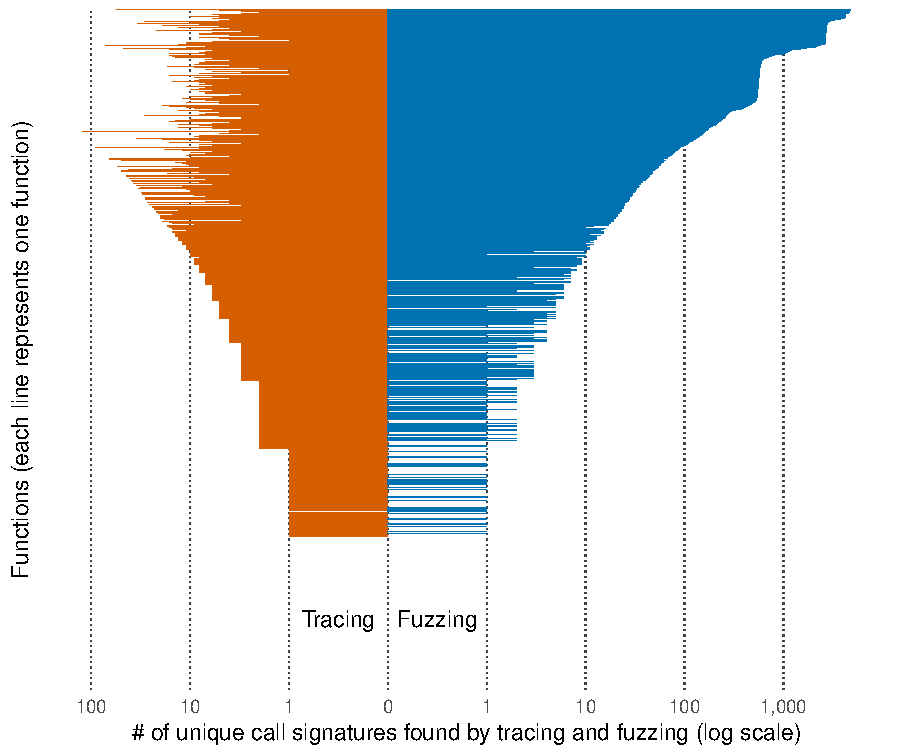
\includegraphics[width=\columnwidth]{code-and-figures/uf-call-signatures.pdf}
    \caption{Number of unique call signatures.}
    \label{fig:call-signatures}
\end{figure}

\section{Conclusions and Future Work}
\label{sec:conclusions}

Fuzz testing is an incredibly useful technique for finding bugs and security vulnerabilities in code, but is hindered by the permissive semantics of dynamic languages as well as the dynamic nature of how complex data is defined.
In this work, we proposed a fuzzing approach that relies on a database of observed values to provide complex and realistic inputs for functions.
We implement this approach in a tool called \tool for the R programming language, and show that \tool uncovers many new and interesting call signatures for R functions.

While this approach was implemented in a tool for R, it is broadly applicable in all languages, and the only real language-specific aspect is the set of parameters in the database.
For instance, one could implement a similar tool for object-oriented languages, where database metadata could include object field names (\Eg, JavaScript).

\bibliographystyle{ACM-Reference-Format}
\bibliography{fuzzing}

\appendix

\section{\tool demonstration}\label{sec:demo}

\lstset{
    basicstyle=\scriptsize\ttfamily,
    numbers=none,
}

The following is a short demonstration of the basic \tool functionality, \Ie how to create the value database by running R code and then how to use it for fuzzing.
The tool is packaged as an R library.
It can be used both in a script or interactively from R REPL.

We begin by starting R (concretely R-dyntrace version 4.0.2) and loading the \tool.
In the following listings, the \code{$} indicates shell prompt and \code{>} denotes the R REPL.

\begin{lstlisting}
$ R
R version 4.0.2 (2020-06-22) -- "Taking Off Again"
...

> library(signatr)
\end{lstlisting}

To generate a database of values, we need some code to run.
One way to get it is to extract it from an existing R package, for example \code{stringr}:

\begin{lstlisting}
> extract_package_code("stringr", output_dir = "demo")
...
 7 examples/str_detect.Rd.R   examples
...
\end{lstlisting}

This will extract all the runnable snippets from the package documentation as
well as tests into the given directory.
For example:

\begin{lstlisting}
$ cat demo/examples/str_detect.Rd.R
...
fruit <- c("apple", "banana", "pear", "pinapple")
str_detect(fruit, "a")
str_detect(fruit, "^a")
...
\end{lstlisting}

Next, we trace the file, \Ie, we execute it and record all the calls using the \code{trace_file} function:

\begin{lstlisting}
> trace_file("demo/examples/str_detect.Rd.R", db_path = "demo.sxpdb")
    status   time   db_size   error
         0  0.024        20      NA
\end{lstlisting}

The result is stored in the \code{demo.sxpdb} database. Concretely, after
running the \code{str_detect.Rd.R} file, it contains 20 unique values. This can
be repeated done for all the other files. To trace multiple files in parallel, we
record each file into its own database and then merge them together using \code{merge_dbs} function.
This also allows us to run larger experiments on multiple machines.

With the database ready, we can start fuzzing.
The fuzzer has a number of configration points, but the easiest is to use \code{quick_fuzz} helper function:

\begin{lstlisting}
> R <- quick_fuzz("stringr::str_detect", "demo.sxpdb", budget = 100, 
                    action = infer_call_signature)

  started a new runner:PROCESS 'R', running, pid 4157
  fuzzing stringr:::str_detect [======] 100/100 (100%) 39s
  stopped runner:PROCESS 'R', running, pid 4157
\end{lstlisting}

The \code{infer_call_signature} is \tool function that uses infers type for each call argument and return value using the type system proposed in Turcotte et al.~\cite{turcotte2020designing}.
The result depends on the action, but in general, it is a data frame with the details of each of the call.
In this case, the data frame includes the inferred call signature in the \code{result} column added there by the \code{infer_call_signature} function.

\begin{lstlisting}
> print(R)
# A tibble: 100 x 6
    args_idx  error                status result               time
    <list>    <chr>                <int>  <chr>                <drtn>
  1 <int [3]> "Error in UseMeth...       1  NA                 0.0363
  2 <int [3]>  NA                        0  (character[],...   0.0351
...
\end{lstlisting}

The above listing shows two calls, a failed one (non-zero status) with an error message, and a successful one with an inferred signature.
The \code{args_idx} contains the indices of the values used from the \sxpdb.

The advantage of being in R is that we can now use all the regular R functions to explore the data.
For example, we can look at the resulting signatures:

\begin{lstlisting}
> count(a, result)
# A tibble: 4 x 2
  result                                                            n
  <chr>                                                         <int>
1 (character[], ^character[], double) => ^logical[]                 1
2 (character[], character, integer) => logical[]                    1
3 (list<integer>, character[], list<integer>) => logical[]          1
4 NA                                                               97
\end{lstlisting}

This shows that in three cases, the fuzzer managed to generate a call that was successful.

\end{document}
\endinput
